\rcsInfo $Id: refinement.tex,v 1.9 2002/12/28 18:43:33 brucker Exp $

\chapter{Discussion: Refining Security Architectures}
In this chapter, we will discuss the conceptual problems of an architectural
refinement and a description of the technology we use to preform our analysis
formally.

\section{Concepts}
As outlined in the previous section, there are conceptually simpler and more
complex architecture models. In a way, one might ask if these models are related
and if this relationship can be used for the task of an analysis.

It is useful to distinguish a \emph{system
  architecture}\index{architecture!system} (which will turn out to be
similar to figure~\ref{fig:overview1}) from a \emph{implementation
  architecture}\index{architecture!implementation} (similar to
figure~\ref{fig:overview3}).  While the former is a model produced
during the system requirements analysis of a software development
process, the latter is merely a product of the design phase
\cite{brohl.ea:vmodell:1995, kruchten:rup:1998}, where the mapping to
a concrete target operating system, programming language and
programming libraries has to be worked out. In the context of
security, this means that conceptually a mapping between these
architecture levels is needed (see figure~\ref{fig:refsec1}).
\begin{figure}
    \center
      \scalebox{0.5}{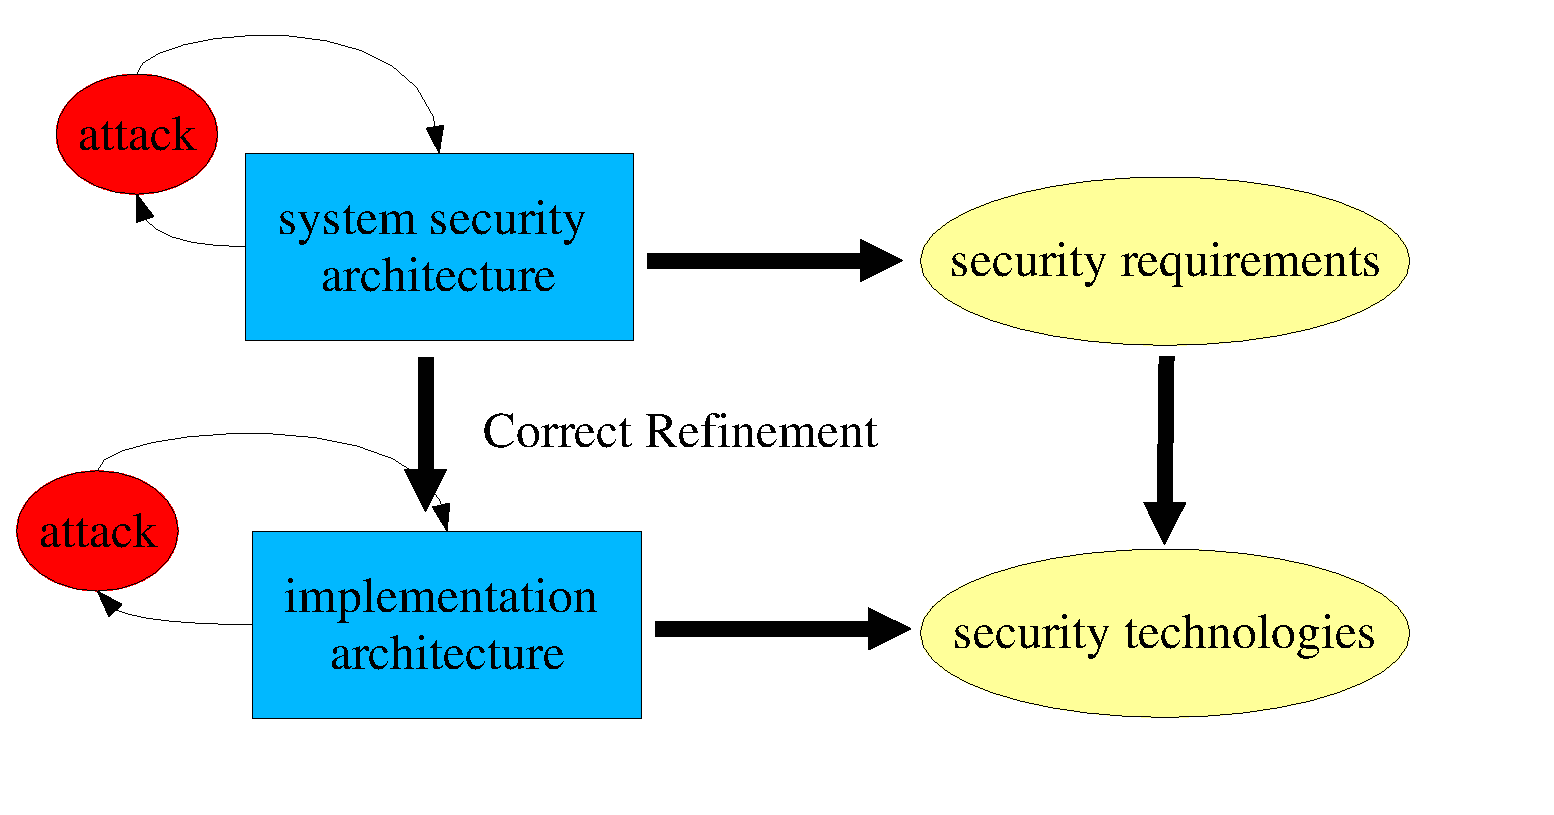
\includegraphics{pics/ref_sec1}}
    \caption{Refining Security Architectures.\label{fig:refsec1}}
\end{figure}
We have a system architecture on top, that is designed to fulfill
certain (security) requirements (a file can only be written, if a
client has an appropriate \emph{role}\index{role}, for example). This
architecture has to be mapped to an implementation architecture with
its security technologies or mechanisms (such as read/write/execute
permissions for files, for example) and security properties (a file
can't be written without write permissions, for example).  Now, we
require the security technology mapping to be correct, i.e.\ the
technologies and their properties meet indeed the security
requirements on the system architecture level.  As an
\emph{attack}\index{attack} we define a sequence of operations, that
attempt to violate a security property; if an architecture ``indeed
meets its security properties'', this means that all attacks have to
be unsuccessful.
  
In the community of formal methods, the relation between abstract and
more concrete views on a system and their semantic underpinning is
well-known under the term \emph{refinement}\index{refinement}, and
security technology mappings can be understood as a special case of
these. Various refinement notions have been proposed (As for Z,
see~\cite{woodcock.ea:using:1996} for example, as for CSP,
see~\cite{roscoe:csp:98}).  In our setting, we chose to use only a
very simple data refinement notion
following~\cite{spivey:z_notation:1992} which essentially requires
that any formula of the abstract view is implied by the formulae of
the concrete view.  Of course, following the approach taken in this
paper, we do not attempt to formally prove such a relationship.
Rather, we will check the consistency of the specifications and their
refinement relation by paper and pencil proofs. In our setting, if the
refinement relation holds, i.e.\ all operations on the concrete layer
indeed preserve the properties of the abstract layer, it can be
concluded for a \emph{correct refinement}, that attacks built by
operations of the abstract layer will not be successful, neither on
the abstract nor the concrete level.
  
Unfortunately, as shown in figure~\ref{fig:refsec2},
\emph{implementing}\index{security implementation} one security
architecture by another opens the door to \emph{new} types of attacks
on the implementation architecture, that can be completely overlooked
on the abstract level.
\begin{figure}
  \center
  \scalebox{0.5}{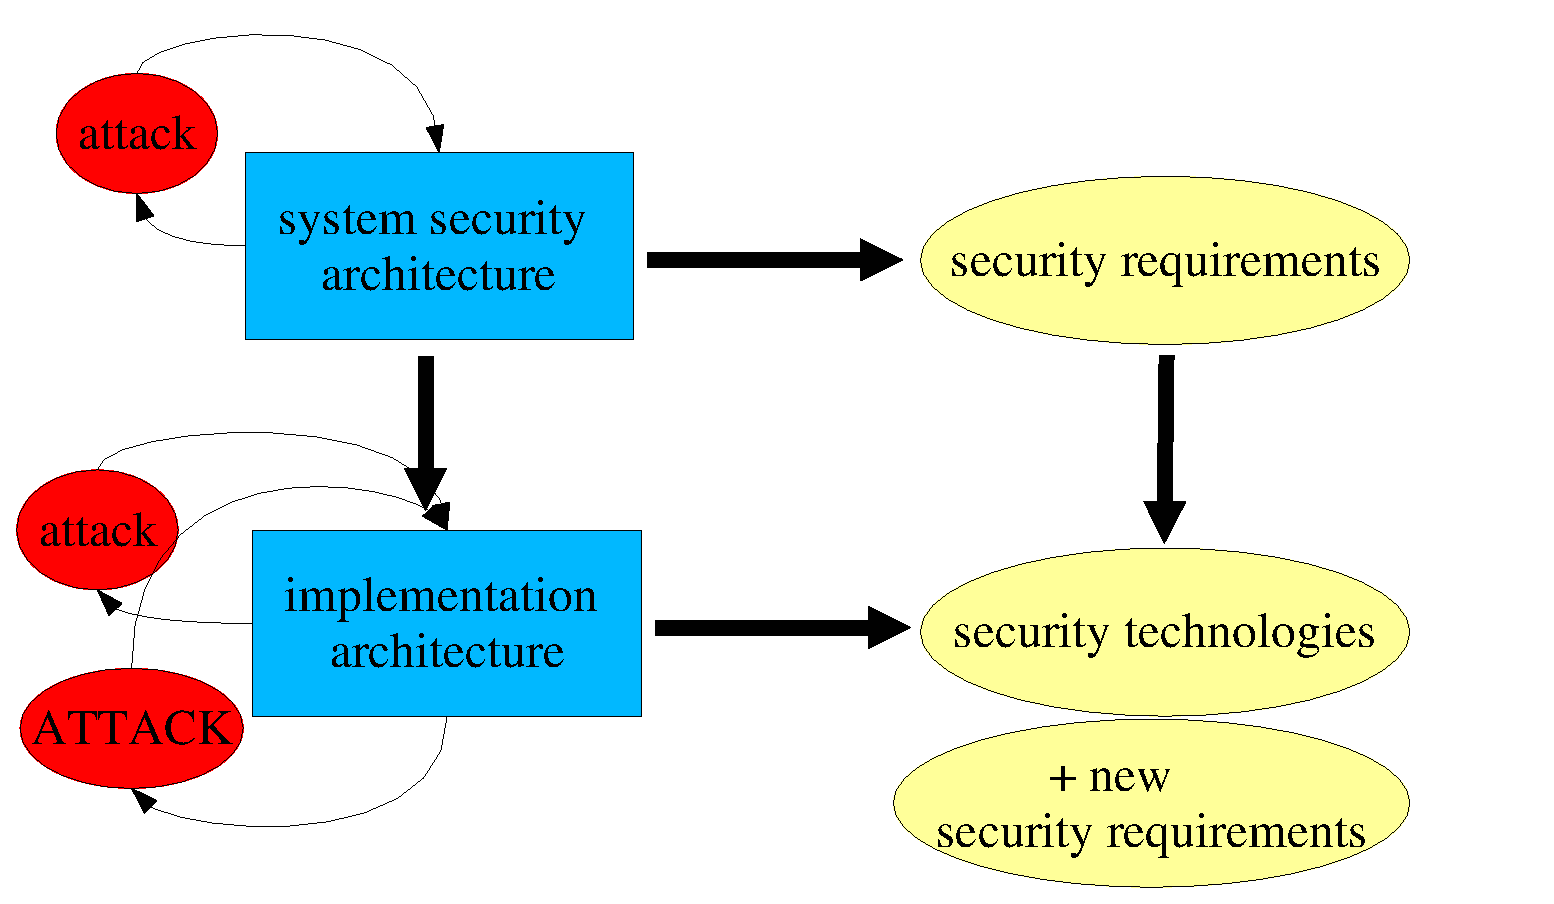
\includegraphics{pics/ref_sec2}}
  \caption{An overview of the open security architecture.\label{fig:refsec2}}
\end{figure}

These new types of attacks\index{attack} may be based on internal data
structures or internal operations of the implementation layer.  The
problem is highly relevant for our case, and, as we believe, for many
practically relevant applications and their security analysis too. In
a way, this reflects common knowledge/experience that implementing an
architecture seems to inherently ``mess up'' a security
concept\index{security concept}.  Maybe that this experience is the
deeper reason for the widespread skepticism against formal
methods\index{formal method} among implementors. However, from the
methodological viewpoint this simply means that \emph{attacks against
  the implementation}\index{attack!implementation} must simply be
taken more seriously, which implies that models of implementation
architectures are deserve more attention as before, where more
abstract models have been preferred.  But in security, more abstract
models are not necessarily better ones.

Coming back to the general refinement scenario, refining an system architecture
be a security technology mapping produces new possibilities of attacks, and
consequently new security requirements on the implementation level.

As an example, consider the instantiation of the previous scheme with our 
application scenario in~\ref{fig:refsec3}.
\begin{figure}
  \center
  \scalebox{0.5}{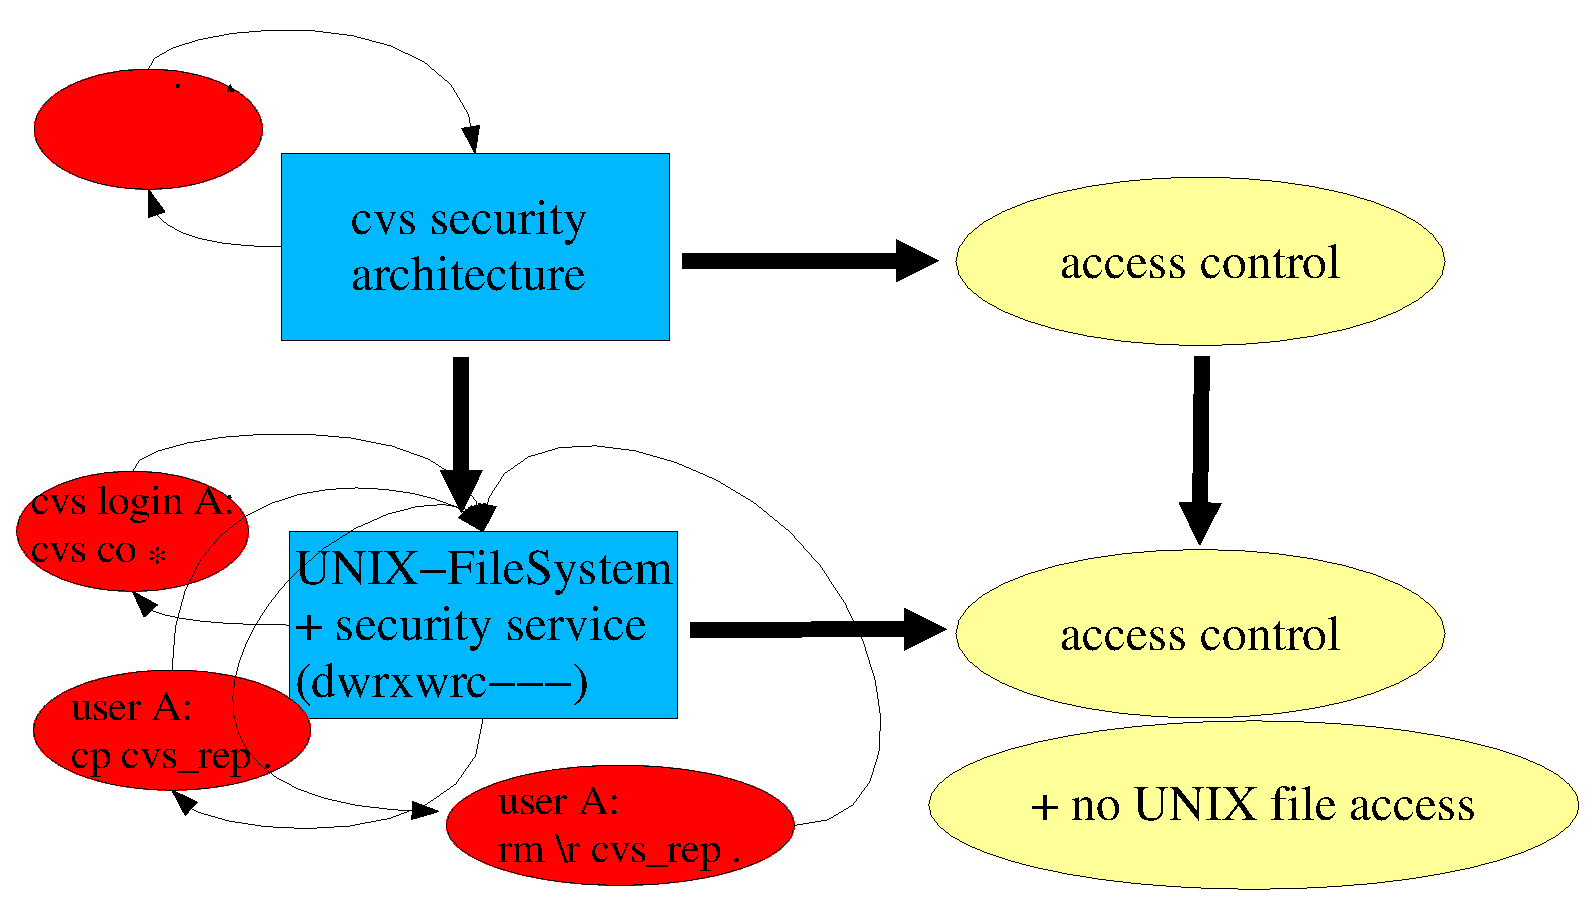
\includegraphics{pics/ref_sec3}}
  \caption{An overview of the open security architecture.\label{fig:refsec3}}
\end{figure}

Using our two-level modeling approach makes it possible to do
security analysis\index{security analysis} on both abstraction levels.
This enables also a combination-strategy of abstract and more concrete
proofs in one setting, allowing to do as much as possible on the
abstract level and concentrating the task on the concrete level to the
parts that deal with implementation specialties that may open the door
for attacks against the implementation.

\section{Performing Refinement Proofs in HOL/Z 2.0}\label{sec:holz}

HOL-Z 2.0\index{HOL-Z} is a tool chain for writing Z specifications,
type-checking them, and proving properties about them. In this
setting, we can specify our Z specifications in a type setting system,
automatically generate proof obligations, import both of them into a
theorem prover environment and use the existing proof mechanisms to
gain a higher degree of automation.  With the proof support for the
schema calculus, realistic analysis of specifications, in particular
refinement proof, in particular proofs along classical data
refinement~\cite{spivey:z_notation:1992} become feasible.

\subsection{HOL-Z: The Tool Chain for Literate Specification}
HOL-Z is now embedded in a chain of tools, that can either be integrated into
XEmacs (the way in which this document was created) or in usual
shell scripts, that allow for an easy integration of the specification process
into the general software development process.
\begin{figure}
\centering\scalebox{.5}{\input{pics/toolchain}}
\caption{A Tool Chain supporting Literate Specification\label{fig:tool-chain-supp}}
\end{figure}
The data flow in our tool chain can be described as follows: At the
beginning, a normal \LaTeX-based Z specification is created. Running
\LaTeX{} leads to the expansion of proof-obligation macros, which also
generates an Isabelle-script\index{Isabelle} that checks that the
obligations are fulfilled (to be run at a later stage).  \Zeta{} takes
over, extracts the definitions and axioms from the \LaTeX{} source
(including the generated ones) and type checks them or provides
animation for some Z schemas.  Our plug-in into \Zeta{} converts the
specification (sections, declarations, definitions, schemas, \ldots)
into SML-files that can be loaded into Isabelle.  In the theory
contexts provided by these files, usual Isabelle proof-scripts can be
developed. An integration of the process into a version management
system allows for semantically checked specifications: for example,
only when the proof obligation check scripts run successfully, new
versions of the specification document are accepted as final versions.

\subsubsection{\texttt{holz.sty} --- A Macro Package for Generating Proof Obligations}
We decided to use \LaTeX{} itself as a flexible mechanism to construct and
present proof-obligations inside the specification --- this may include
consistency conditions, refinement conditions or special safety properties
imposed by a special formal method for a certain specification architecture. Our
\LaTeX-package \verb|holz.sty| provides, among others, commands for generating
refinement conditions as described in~\cite{spivey:z_notation:1992},
where also the paradigmatical ``BirthdayBook'' is presented we use as running 
example. For $AddBirthday$ \emph{is refined by} $AddBirthday1$, we instantiate 
a macro as follows:
{\small
\begin{verbatim}
\zrefinesOp[Astate=BirthdayBook, Cstate=BirthdayBook1,
            Aop=AddBirthday, Cop=AddBirthday1,
            Args={name?: NAME; date?: DATE}, Abs=Abs]{Add}
\end{verbatim}
Here, \verb|Astate| contains the schema describing the abstract
state and \verb|Cstate| hold the schema describing the concrete state. Based
on this input, our \LaTeX-package automatically generates the following two
proof obligations:
\begin{zed}
Add_1 &==& \forall BirthdayBook;  BirthdayBook1; name?: NAME; date?: DATE @ \\
&&(\pre AddBirthday \land Abs) \implies \pre AddBirthday1\\
Add_2 &==& \forall BirthdayBook;  BirthdayBook1;  BirthdayBook1 ';name?: NAME;\\
&& date?: DATE @ (\pre AddBirthday \land Abs \land AddBirthday1)\\
&&\implies(\exists BirthdayBook ' @ Abs ' \land AddBirthday)\\ 
\end{zed}
These proof obligations are type checked using \Zeta{} and are converted to
\holz{} by our \Zeta{}-to-\holz converter. 

\subsubsection{The \Zeta-System}
\Zeta~\cite{zeta}\index{Zeta@{\Zeta}} is an open environment for the development, analysis and
animation of specifications based on Z. Specification documents are represented
by \emph{units} in the \Zeta{} system, that can be annotated with different
\emph{content} like \LaTeX{} mark-up, type-checked abstract syntax, etc. The
contents of units is computed by adaptors, which can be plugged into the system
dynamically.


\subsubsection{\Zeta-to-\holz{}Converter}
The converter consists of two parts: an adaptor that is plugged into \Zeta and
converts the type-checked abstract syntax of a unit more or less directly into an
SML file. On the SML side, this file is read and a theory context is build
inside Isabelle/HOL-Z. This involves an own type-checking and an own check of
integrity conditions of the specification and some optimizations for partial
function application in order to simplify later theorem proving.


\subsection{Proof Support for Z}
\subsubsection{Isabelle/HOL-Z revisited}
The language Z is centered around a specific structuring mechanism
called \emph{schema}\index{schema}. Semantically, schemas are just
sets of records (called \emph{bindings}\index{binding} in Z
terminology;~\cite{iso:z:2000}) of a certain type.  Z is based on
typed set theory equivalent to HOL set theory. However, a reference to
a schema can play different \emph{roles} in a specification: it can
serve as \emph{import} in the declaration list in other schemas, or as
\emph{predicate} (where all arguments are suppressed syntactically),
or as \emph{set} (see~\cite{kolyang.ea:z:96} for more details).

The approach of HOL-Z is to represent records by products in Isabelle/HOL and to
manage their layout in order to support \emph{as import}-references. This is
achieved by a parser making implicit bindings in Z expressions explicit and
generating coercions of schemas according to their role. For example, we assume
throughout this section a schema $A$ of type $[ x_1 \bindsto \tau_1, x_2
\bindsto \tau_2]$ and a schema $B$ of type $[ x_2 \bindsto \tau_2, x_3 \bindsto
\tau_3]$. Then, a schema expression $A \land B$ can be represented by
\[ \lambda (x_1,x_2,x_3)\bullet A(x_1,x_2) \land B(x_2,x_3)\;, \]
while an expression $A \cup A$ will be represented by 
$(\mathrm{asSet}~A) \cup (\mathrm{asSet}~A)$.

Thus, having ``parsed away'' the specific binding conventions of Z into standard
$\lambda$-calculus, Isabelle's proof-engine can handle Z as ordinary
HOL-formulas. There is no more ``embedding specific'' overhead such as
predicates stating the well-typedness of certain expressions, etc.

For full-automatic proofs this is fine; however, in practice, realistic case
studies require proofs with user interaction. This leads to the requirement that
intermediate lemmas can be inserted ``in the way of Z'', intermediate results
are presented ``Z-alike'' and deduction attempts to mimic the proof style
imposed by Z (cf.~\cite{woodcock.ea:using:1996}). As a prerequisite, we defined
a special abstraction operator \emph{SB} semantically equivalent to the
pair-splitting $\lambda$-abstraction from the example above, which is actually
encoded by:
\[
  \mathrm{SB}~\mbox{``$x_1$''} \leadsto x_1, \mbox{``$x_2$''} \leadsto x_2, 
  \mbox{``$x_3$''} \leadsto x_3\bullet A(x_1,x_2) \land B(x_2,x_3) 
\]
where each field-name is kept as a (semantically irrelevant) string in the
representation. Thus, while the ``real binding'' is dealt with by Isabelle's
internal $\lambda$, which is underlying $\alpha$-conversion, the
\emph{presentation} of intermediate results is done on the basis of the original
field-names used in the users specification.

\subsubsection{New Proof Support in HOL-Z 2.0}
Schemas can also be used in quantifications as part of some very Z specific
concept, the so-called \emph{schema calculus}, for which we implemented syntax 
and proof support. For
example, $\forall A \spot B$ is a schema of type $\power ([x_3 \bindsto
\tau_3])$. In HOL-Z, it is represented by:
\[ 
  \mathrm{SB}~\mbox{''$x_3$''} \leadsto x_3\bullet \forall (x_1,x_2) :
  \mathrm{asSet}~A \spot B(x_2,x_3) 
\]
This and similar quantifiers and operators allow for a very compact presentation
of typical proof-obligations occurring in refinements in Z. As example, we use 
an already slightly simplified version of $Add_1$ already described 
in~\cite[pp. 138]{spivey:z_notation:1992}. (The full proof had been omitted 
for space reasons). Instead of referring to constants representing the proof 
obligations generated by the \LaTeX-based front-end, we use the HOL-Z-parser directly:
\begin{holzverb}
zgoal thy 
"%A BirthdayBook @  %A  BirthdayBook1 @  %A  name? %:  Name @ %A date? %:  Date @ 
      (name? ~:  known /\  known = {n. ?i: #1..hwm. n=names %^ i}
       =+=> (!i : #1..hwm. name? ~=  names %^ i))";
\end{holzverb}
which opens an Isabelle proof-state.

In the literature, several calculi for the schema calculus have been presented
more or less formally (\cite{iso:z:2000,henson.ea:logic:1998}). From the
perspective of HOL-Z it is quite clear what is needed: for any construct of the
schema calculus, a special tactic must be provided that works analogously to the
usual introduction and elimination rules for standard (bounded) quantifiers and
set comprehensions. These tactics have been implemented and combined to new
tactics, for example to a tactic that ``strips-off'' all universal quantifiers
(including schema quantifiers) and implications. Thus, the HOL-Z tactic:
\begin{holzverb}
   by(stripS_tac 1);
\end{holzverb}
transforms the goal into the following proof state:
\begin{holzverb}
1. !!birthday known dates hwm names name? date? i.
    [| BirthdayBook (birthday, known); BirthdayBook1 (dates, hwm, names);
       name? : Name; date? : Date;
       name? ~:  known /\  known = {n. ?i: #1..hwm. n=names %^ i};
       i : ( #1 .. hwm) |] ==> name? ~=  names %^ i
\end{holzverb}
Note that the quite substantial reconstruction of the underlying binding still
leads to a proof state that is similar in style and presentation
to~\cite{woodcock.ea:using:1996}.

Besides the ``schema calculus'', Z comes with a large library of set operators
specifying relations, functions as relations, sequences and bags; this library
--- called the \emph{Mathematical Toolkit} of Z --- differs in style
substantially from the Isabelle/HOL library, albeit based on the same
foundations. For HOL-Z 2.0, we improved this library substantially and added
many derived rules that make a higher degree of automatic reasoning by
Isabelle's standard proof procedures possible. For example, the goal above is
simply ``blown away'' by:
\begin{holzverb}
   auto();
\end{holzverb}
which finishes the proof.
%%% Local Variables:
%%% TeX-master: "arch"
%%% fill-column:80
%%% x-symbol-8bits:nil
%%% End:
